%%%%%%%%%%%%%%%%%%%%%%%%%%%%%%%%%%%%%%%%%
% a0poster Landscape Poster
% LaTeX Template
% Version 1.0 (22/06/13)
%
% The a0poster class was created by:
% Gerlinde Kettl and Matthias Weiser (tex@kettl.de)
% 
% This template has been downloaded from:
% http://www.LaTeXTemplates.com
%
% License:
% CC BY-NC-SA 3.0 (http://creativecommons.org/licenses/by-nc-sa/3.0/)
%
%%%%%%%%%%%%%%%%%%%%%%%%%%%%%%%%%%%%%%%%%

%----------------------------------------------------------------------------------------
%	PACKAGES AND OTHER DOCUMENT CONFIGURATIONS
%----------------------------------------------------------------------------------------

\documentclass[a0,landscape]{a0poster}

\usepackage{multicol} % This is so we can have multiple columns of text side-by-side
\columnsep=100pt % This is the amount of white space between the columns in the poster
\columnseprule=7pt % This is the thickness of the black line between the columns in the poster

\usepackage[svgnames]{xcolor} % Specify colors by their 'svgnames', for a full list of all colors available see here: http://www.latextemplates.com/svgnames-colors

\usepackage{times} % Use the times font
%\usepackage{palatino} % Uncomment to use the Palatino font

\usepackage{graphicx} % Required for including images
\graphicspath{{figures/}} % Location of the graphics files
\usepackage{booktabs} % Top and bottom rules for table
\usepackage[font=large,labelfont=bf]{caption} % Required for specifying captions to tables and figures
\usepackage{amsfonts, amsmath, amsthm, amssymb} % For math fonts, symbols and environments
\usepackage{wrapfig} % Allows wrapping text around tables and figures
\usepackage{comment}
\usepackage{bm}
\usepackage{anyfontsize}
\usepackage{multirow}

\usepackage[margincaption,outercaption,raggedright,wide]{sidecap}
\sidecaptionvpos{table}{t}

\usepackage{fancyvrb}
\DefineVerbatimEnvironment{pycode}{BVerbatim}{baseline=t}

\newcommand{\mysection}[1]{\section*{\fontsize{67.1}{82} \selectfont \color{NavyBlue} #1 \color{Black}}}

\usepackage{subfigure}

\usepackage{parskip}

\usepackage{url}

\usepackage{float} 

\renewcommand{\vec}[1]{{\boldsymbol{\mathbf{#1}}}} % vector
\newcommand{\mat}[1]{{\ensuremath{\mathbf{#1}}}} % matrix

\newcommand{\R}{\mathbb{R}}
\newcommand{\E}{\mathbb{E}}
\newcommand{\Loss}{\mathcal{L}}
\newcommand{\loss}{\ell}
\newcommand{\sample}{\sim}
\DeclareMathOperator*{\argmin}{argmin}
\DeclareMathOperator*{\argmax}{argmax}

\newcommand{\code}{\texttt}
\newcommand{\sectionx}{\textbf}

\begin{document}

%----------------------------------------------------------------------------------------
%	POSTER HEADER 
%----------------------------------------------------------------------------------------

% The header is divided into three boxes:
% The first is 55% wide and houses the title, subtitle, names and university/organization
% The second is 25% wide and houses contact information
% The third is 19% wide and houses a logo for your university/organization or a photo of you
% The widths of these boxes can be easily edited to accommodate your content as you see fit

\begin{centering}{\fontsize{100}{120} \selectfont \color{NavyBlue} \textbf{The Machine Learning Benchmark Tools Package} \color{Black}}\\ % Title
%
\includegraphics[width=10cm]{uber_ai_logo_bootleg.pdf} \\ % TODO try and move this to the right?
\Huge \textbf{Ryan Turner}\\ % Author(s)
\end{centering}

\vspace{1cm} % A bit of extra whitespace between the header and poster content

%----------------------------------------------------------------------------------------

\begin{multicols}{3} % This is how many columns your poster will be broken into, a poster with many figures may benefit from less columns whereas a text-heavy poster benefits from more

%----------------------------------------------------------------------------------------
%	INTRODUCTION
%----------------------------------------------------------------------------------------

\Large

\mysection{Introduction}

\begin{itemize}
  \item Easy benchmarking of machine learning models with sklearn interface with statistical tests built-in
  \item Error bars and significance tests should be standard in ML
  \item One liner on sklearn compatible objects: 
  \begin{itemize}
    \item train, test, and evaluate the models on multiple loss functions
  \end{itemize}
  \item Process is usable in a modular way
\end{itemize}

\begin{itemize}
  \item Multiple loss functions is a key design principle
  \item Bayes' decision rule: predictive distn.~$\rightarrow$ \emph{action} for each loss function
  \item \textbf{Example}: MSE $\implies$ mean, MAE $\implies$ median
  \item Automatic conversion to ensure model fairly compared across metrics
\end{itemize}
%
\textbf{Code}
\large {\url{github.com/rdturnermtl/benchmark_tools}}

\columnbreak

\mysection{The interface}
%
\begin{itemize}
  \item Classication uses \code{benchmark\_tools.classification}
  \item Regression uses \code{benchmark\_tools.regression}
  \item Bayes' decision rule converts predictive distribution to \emph{action} for each loss function
  \item Objects just support methods \code{fit} and \code{predict\_log\_proba} (sklearn interface)
\end{itemize}
%
\sectionx{Modular pieces}
\begin{itemize}
  \item ``do-it-all'' \code{just\_benchmark} routine has 3 phases
  \item \code{get\_pred\_log\_prob}: predictive distributions on each test point and model
  \item \code{loss\_table}: the losses for each prediction
  \item \code{loss\_summary\_table}: mean loss for each method $+$ error bars and p-values
\end{itemize}
%
\sectionx{Sciprint}
\begin{itemize}
  \item Publishable results: one must first format \code{performance\_df}
  \item Cleanly format: correct significant figures, shifting of exponent for compactness, and correct alignment of decimal points, units in headers
\end{itemize}
%
\sectionx{Data splitter}
\begin{itemize}
  \item Supports random, ordinal, or temporal splitting across features in pandas dataframes
  \item Jointly splitting across multiple features to test difficult generalization cases
\end{itemize}

\columnbreak

\mysection{Evaluation framework}

\begin{itemize}
  \item Two metric types: \emph{loss functions} and \emph{curve summaries}
  \begin{align}
    \Loss_A = \frac{1}{N} \sum_{i=1}^N \loss_i = \frac{1}{N} \sum_{i=1}^N \loss(y_i, a_i)\,, \quad a_i = \argmin_a \E_{P_A(y_i|\vec x_i)}[\loss(y_i, a)]
  \end{align}
  \item Curve summaries (ROC, PR, PRG) for a single number
  \item Built-in \emph{proper scoring rules}: log loss (NLL), Brier loss, spherical loss
  \item General loss matrices, and new metrics are easily added
  \item Non-probabilistic methods usable by ``pipelining'' a \emph{calibrator}
\end{itemize}

\sectionx{Error bars and significance tests}
\begin{itemize}
  \item Place CI on mean loss with $N \rightarrow \infty$ test set from the same distn.
  \item Three methods for CI: t-test, bootstrap, and Bernstein bound
  \item p-values designed to match the error bars (can be via the 3 methods)
\end{itemize}

\sectionx{Error bars on curves}
\begin{itemize}
  \item CI on raw curves (for plotting) and AUC (for tables) via bootstrap
  \item Vectorized bootstrap: reweight data points via multinomial distribution
  \item Avoids re-creating the data sets in memory (very slow)
\end{itemize}

\end{multicols}

\vspace{5mm}
\hrule
\vspace{5mm}

\begin{multicols}{2}

\Large

\mysection{Examples}

\begin{itemize}
  \item Motivation: reduce common ``boilerplate'' code across ML projects
  \item Pipeline: split data, training models, testing models, evaluating/statistical analysis, and formatting of tables
  \item Just two phases: \code{just\_benchmark} and \code{just\_format\_it}
\end{itemize}

\sectionx{Classification}
{\normalsize
\begin{verbatim}
import benchmark_tools.classification as btc
from benchmark_tools.classification import STD_CLASS_LOSS, STD_BINARY_CURVES
performance_df, performance_curves_dict = \
    btc.just_benchmark(X_train, y_train, X_test, y_test, 2, classifiers,
                       STD_CLASS_LOSS, STD_BINARY_CURVES, ref_method='iid')
\end{verbatim}
}
The \code{classifiers} dictionary is as simple as:
{\normalsize
\begin{verbatim}
classifiers = {'iid': btc.JustNoise(),
               'Nearest Neighbors': KNeighborsClassifier(3),
               'Linear SVM': SVC(kernel='linear', C=0.025, probability=True),
               'RBF SVM': SVC(gamma=2, C=1, probability=True)}
\end{verbatim}
}
\begin{itemize}
  \item Loss functions in \code{STD\_CLASS\_LOSS}, curves (e.g., ROC, PR) in \code{STD\_BINARY\_CURVES}
  \item \code{ref\_method} reference for paired statistical tests
  \item Constant prediction dummy model in \code{JustNoise}
\end{itemize}
{\normalsize
\begin{verbatim}
import benchmark_tools.sciprint as sp
print(sp.just_format_it(performance_df, shift_mod=3, unit_dict={'NLL': 'nats'},
                        non_finite_fmt={sp.NAN_STR: '{--}'}, use_tex=True))
\end{verbatim}
}
\begin{center}
{\footnotesize
\setlength{\tabcolsep}{0.75em} % for the horizontal padding
\begin{tabular}{|l|l|r|l|r|l|r|l|r|l|r|l|r|l|r|}
\toprule
{}                &       {AP} &      {p} &      {AUC} &      {p} &  {AUPRG} &      {p} &    {Brier} &      {p} & {NLL (nats)} &      {p} &   {sphere} &      {p} & {zero one} &      {p} \\
\midrule
%AdaBoost          &  0.93(16)  &  $<$0.0001 &  0.950(96) &  $<$0.0001 &  0.90464 &  $<$0.0001 &  0.42(14)  &  $<$0.0001 &    0.368(80) &  $<$0.0001 &  0.36(15)  &  $<$0.0001 &  0.075(86) &  $<$0.0001 \\
%Decision Tree     &  0.95(13)  &  $<$0.0001 &  0.966(70) &  $<$0.0001 &  0.93860 &  $<$0.0001 &  0.18(25)  &  $<$0.0001 &    0.40(71)  &   0.4072 &  0.16(22)  &  $<$0.0001 &  0.050(71) &  $<$0.0001 \\
%Gaussian Process  &  0.90(22)  &  $<$0.0001 &  0.95(12)  &  $<$0.0001 &  0.92081 &  $<$0.0001 &  0.27(17)  &  $<$0.0001 &    0.27(11)  &  $<$0.0001 &  0.22(16)  &  $<$0.0001 &  0.025(51) &  $<$0.0001 \\
Linear SVM        &  0.952(99) &  $<$0.0001 &  0.950(77) &  $<$0.0001 &  0.88705 &  $<$0.0001 &  0.34(24)  &  $<$0.0001 &    0.29(16)  &  $<$0.0001 &  0.31(24)  &  $<$0.0001 &  0.15(12)  &   0.0006 \\
%Naive Bayes       &  0.957(97) &  $<$0.0001 &  0.957(68) &  $<$0.0001 &  0.89782 &  $<$0.0001 &  0.34(25)  &  $<$0.0001 &    0.28(18)  &  $<$0.0001 &  0.31(24)  &  $<$0.0001 &  0.13(11)  &   0.0002 \\
Nearest Neighbors &  0.94(14)  &  $<$0.0001 &  0.969(69) &  $<$0.0001 &  0.93498 &  $<$0.0001 &  0.18(21)  &  $<$0.0001 &    0.42(70)  &   0.4241 &  0.15(18)  &  $<$0.0001 &  0.025(51) &  $<$0.0001 \\
%Neural Net        &  0.957(91) &  $<$0.0001 &  0.957(69) &  $<$0.0001 &  0.89782 &  $<$0.0001 &  0.33(23)  &  $<$0.0001 &    0.28(15)  &  $<$0.0001 &  0.30(22)  &  $<$0.0001 &  0.100(98) &  $<$0.0001 \\
%QDA               &  0.951(91) &  $<$0.0001 &  0.950(80) &  $<$0.0001 &  0.88517 &  $<$0.0001 &  0.34(27)  &  $<$0.0001 &    0.29(21)  &   0.0003 &  0.31(25)  &  $<$0.0001 &  0.15(12)  &   0.0006 \\
RBF SVM           &  0.93(18)  &  $<$0.0001 &  0.957(94) &  $<$0.0001 &  0.92081 &  $<$0.0001 &  0.14(20)  &  $<$0.0001 &    0.18(18)  &  $<$0.0001 &  0.12(17)  &  $<$0.0001 &  0.025(51) &  $<$0.0001 \\
%Random Forest     &  0.965(82) &  $<$0.0001 &  0.949(84) &  $<$0.0001 &  0.92147 &  $<$0.0001 &  0.31(26)  &  $<$0.0001 &    0.52(70)  &   0.6099 &  0.28(24)  &  $<$0.0001 &  0.100(98) &  $<$0.0001 \\
iid               &  0.53(16)  &     {--} &  0.5(0)    &     {--} &  0(0)    &     {--} &  1.004(22) &     {--} &    0.695(11) &     {--} &  1.005(27) &     {--} &  0.53(17)  &     {--} \\
\bottomrule
\end{tabular}
}
\end{center}

\columnbreak

\sectionx{Performance curves}

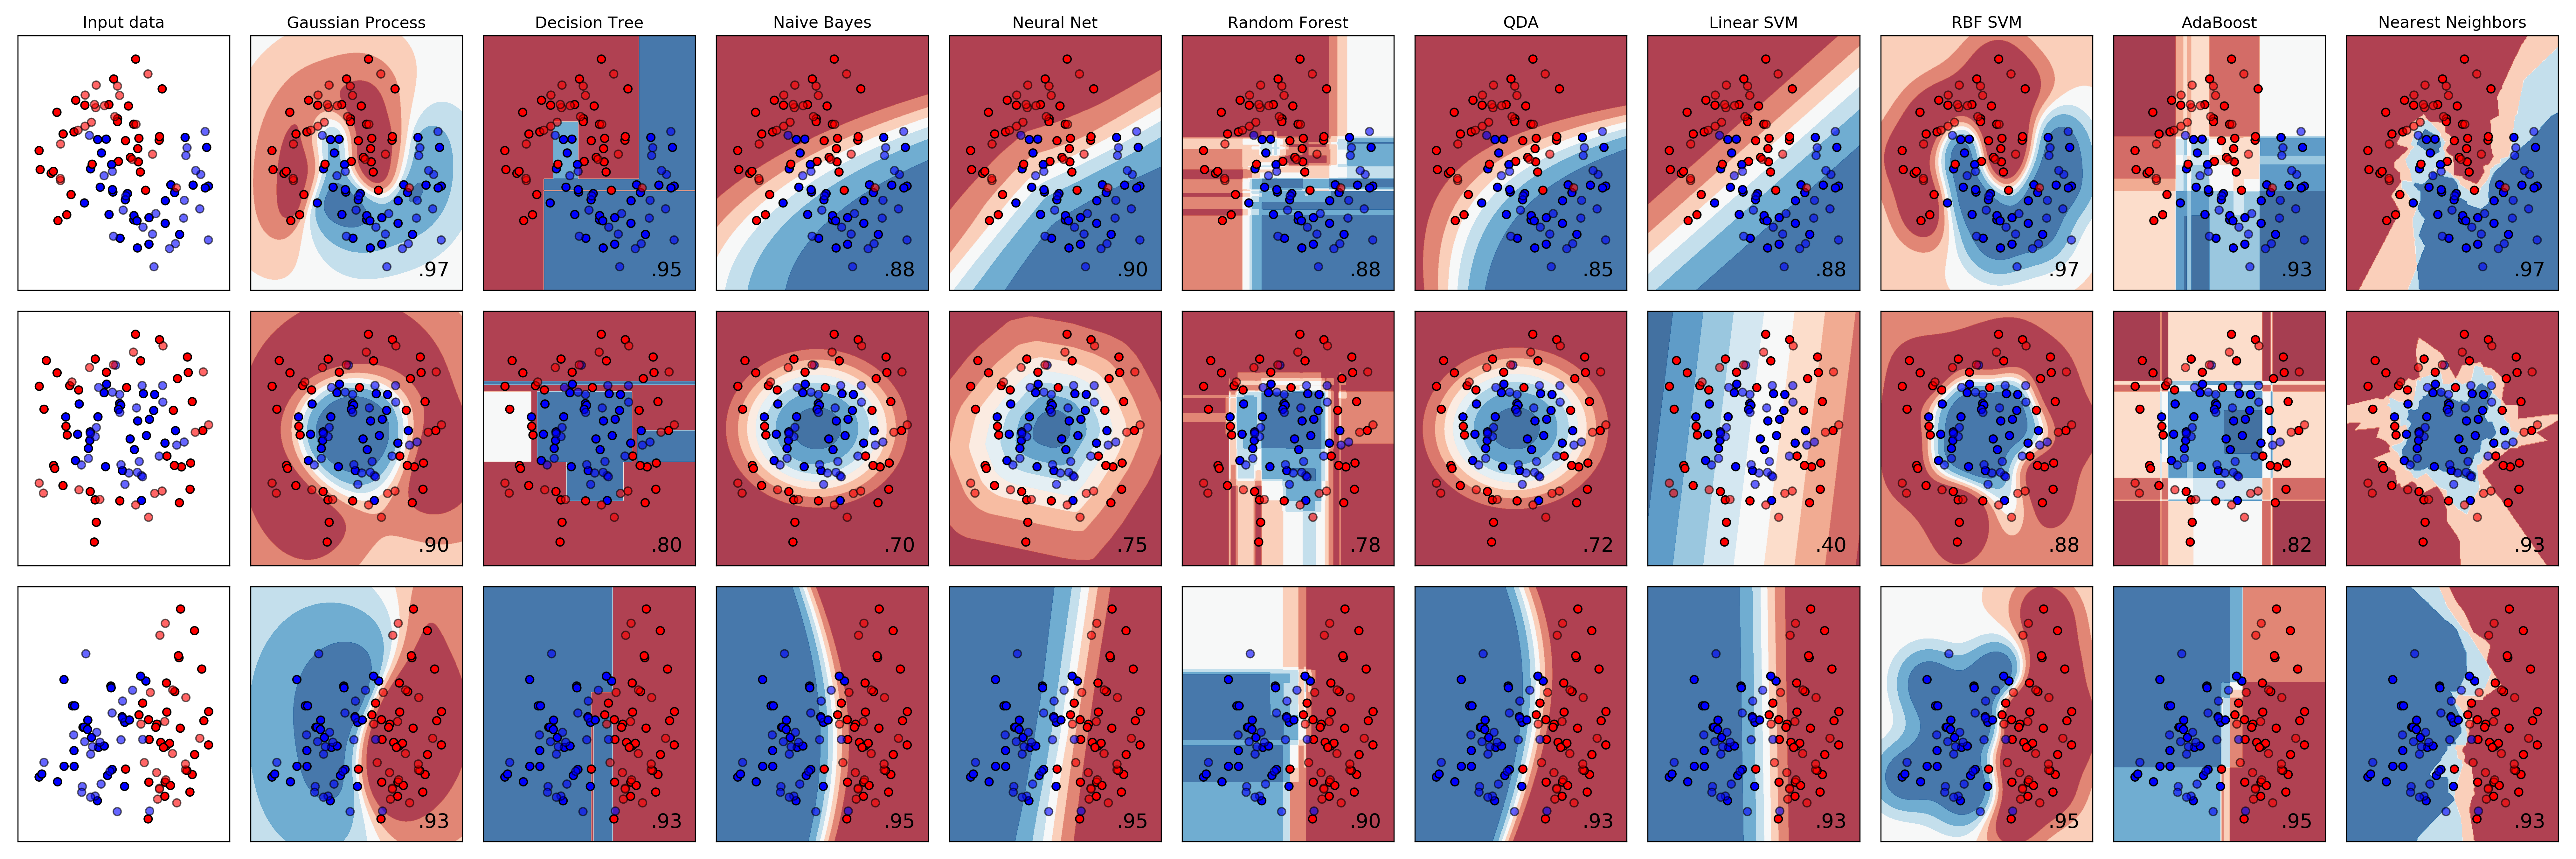
\includegraphics[width=0.4\textwidth]{output.png}\\
\begin{minipage}[b][2.7in][c]{1.6in}
ROC
\end{minipage}
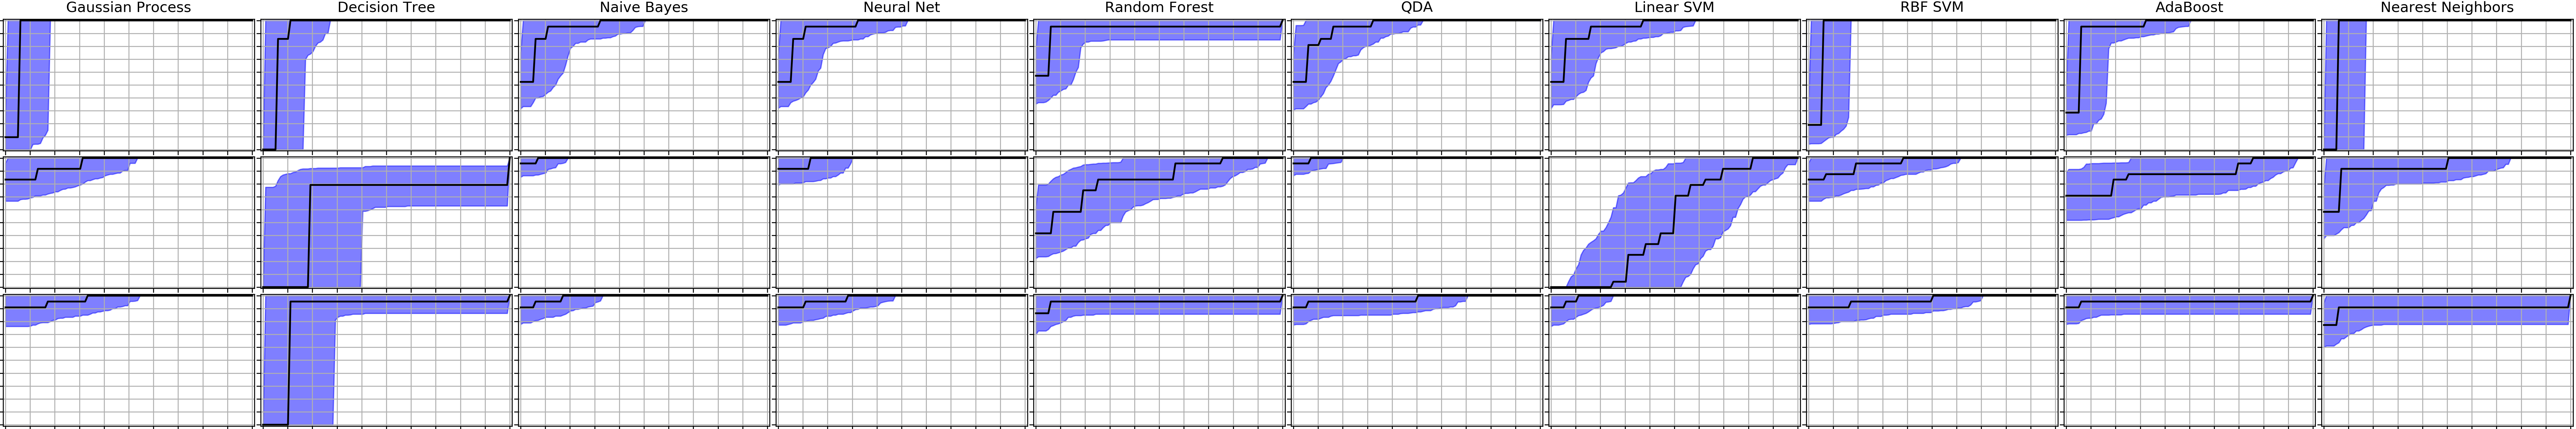
\includegraphics[width=0.36\textwidth]{AUC.png}\\
\begin{minipage}[b][2.7in][c]{1.6in}
PR
\end{minipage}
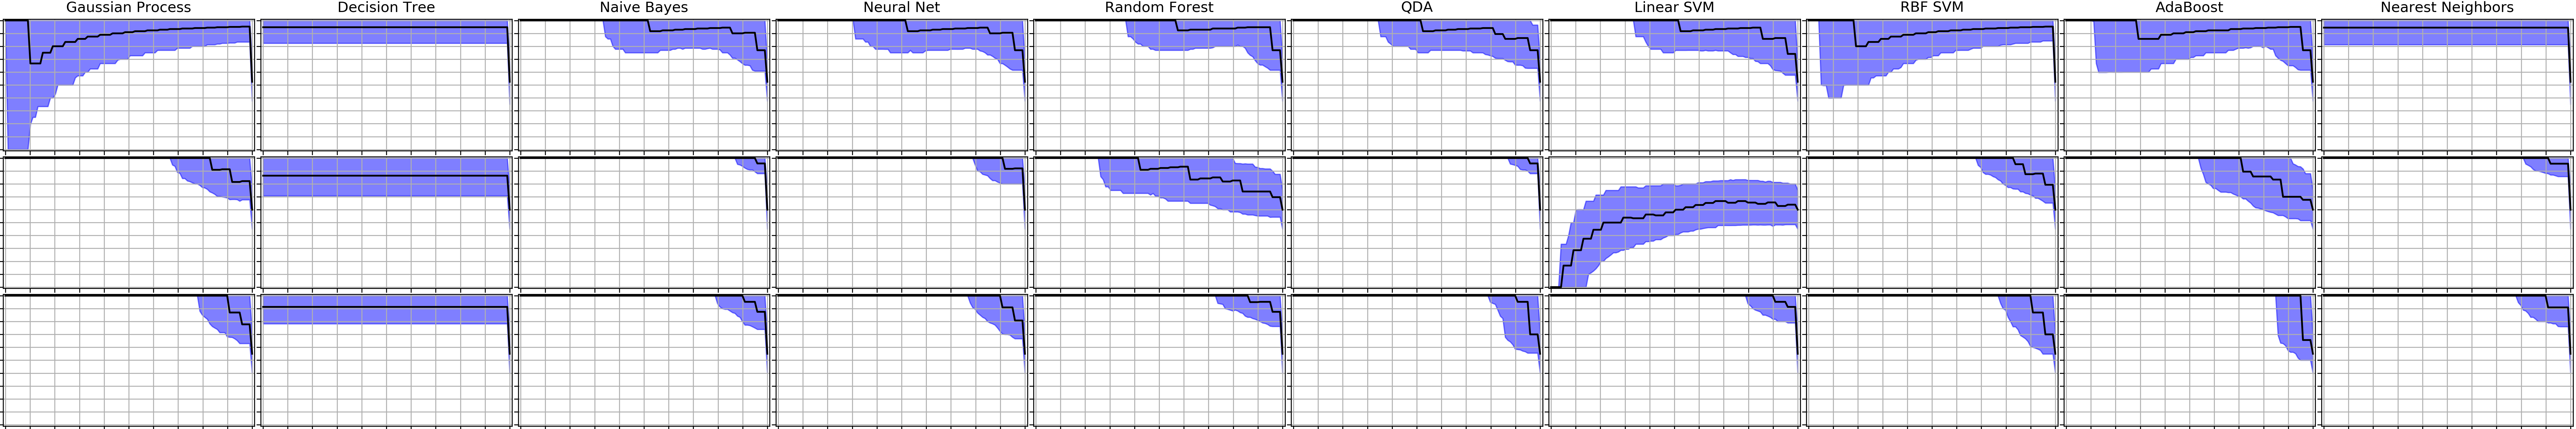
\includegraphics[width=0.36\textwidth]{AP.png}

\sectionx{Regression}

\vspace{-1cm}

{\normalsize
\begin{tabular}{cc}
\begin{pycode}
import benchmark_tools.regression as btr
full_tbl = btr.just_benchmark(X_train, y_train, X_test, y_test,
                              regressors, STD_REGR_LOSS, 'iid',
                              pairwise_CI=True)
\end{pycode}
&
{\footnotesize
\begin{tabular}{|l|l|r|l|r|l|r|}
\toprule
{}  &        {MAE} &     {p} &        {MSE} &      {p} & {NLL (nats)} &      {p} \\
\midrule
BLR &  0.96933(30) &  0.0979 &  1.39881(67) &   0.0665 &  1.58842(57) &   0.9828 \\
GPR &  0.75(13)    &  0.0009 &  0.75(28)    &  $<$0.0001 &  1.27(12)    &  $<$0.0001 \\
iid &  0.96908     &    {--} &  1.3982      &     {--} &  1.5884      &     {--} \\
\bottomrule
\end{tabular}
}
\end{tabular}
}

\end{multicols}

\end{document}

